\subsection{Comparaison Value Iteration et Policy Iteration}
\label{sec:c:comparison}

\paragraph{Protocole de comparaison}
Les deux algorithmes sont lanc\'{e}s avec les m\^{e}mes param\`{e}tres
($\gamma$, $\varepsilon$) sur le m\^{e}me MDP PlateVision ($N=7$, $A=5$).
Le temps de calcul est mesur\'{e} par chronom\'{e}trage wall-clock
(\texttt{time.perf\_counter()}).

\begin{table}[H]
\centering
\caption{Comparaison VI vs PI --- convergence et accord politique ($\varepsilon=0.01$)}
\label{tab:c:vi_pi_comparison}
\begin{tabular}{rrrrrr}
\toprule
$\gamma$ & VI it\'{e}r. & PI it\'{e}r. & VI t (s) & PI t (s) & Accord $\pi^*$ \\
\midrule
  0.50 & 17 & 2 & 0.0001 & 0.0004 & 100% \\
  0.70 & 32 & 2 & 0.0002 & 0.0007 & 100% \\
  0.80 & 50 & 2 & 0.0003 & 0.0009 & 100% \\
  0.90 & 105 & 3 & 0.0006 & 0.0039 & 100% \\
  0.95 & 281 & 4 & 0.0031 & 0.0094 & 100% \\
  0.99 & 1493 & 4 & 0.0094 & 0.0445 & 100% \\

\bottomrule
\end{tabular}
\end{table}

\paragraph{Explication th\'{e}orique}
\textbf{Value Iteration} (VI) applique l'op\'{e}rateur de Bellman
jusqu'\`{a} ce que les valeurs convergent ($\Delta V < \varepsilon$).
Le nombre d'it\'{e}rations cro\^{i}t avec $\gamma$ car le rayon spectral
de l'op\'{e}rateur de contraction vaut $\gamma$ : un $\gamma$ plus \'{e}lev\'{e}
ralentit la propagation de l'information.
\textbf{Policy Iteration} (PI) alt\`{e}rne \'{e}valuation exacte de
$V^{\pi}$ et am\'{e}lioration greedy. Chaque it\'{e}ration de politique
est garantie monotone (le th\'{e}or\`{e}me d'am\'{e}lioration de politique
--- Russell \& Norvig, Ch.~17.3) --- PI converge donc en
\textbf{4} it\'{'}ration(s) globale(s) contre \textbf{281} pour VI
\`{a} $\gamma=0.95$.

\paragraph{R\'{e}sultat}
Les deux algorithmes produisent une politique $\pi^*$ identique à 100\,\%
(taux d'accord $\pi^*_{{\text{{VI}}}} = \pi^*_{{\text{{PI}}}}$).
Ce r\'{e}sultat confirme la robustesse de la solution MDP : ind\'{e}pendamment
de la m\'{e}thode de r\'{e}solution, l'action optimale par \'{e}tat est
univoque.

\paragraph{Recommandation d\'{e}ploiement MINT/DGI}
Pour un d\'{e}ploiement en production :
\begin{itemize}
\item \textbf{Petit espace d'\'{e}tats ($N \leq 50$) :} Policy Iteration
      recommand\'{e}e --- convergence quasi-instantan\'{e}e, facilit\'{e}
      de re-calibration lors de mises \`{a} jour des matrices $P$ ou $R$.
\item \textbf{Grand espace d'\'{e}tats ($N > 1000$) :} Value Iteration
      pr\'{e}f\'{e}r\'{e}e --- chaque it\'{e}ration PI n\'{e}cessite
      une r\'{e}solution de syst\`{e}me lin\'{e}aire de taille $N^2$.
\end{itemize}

\begin{figure}[H]
\centering
\IfFileExists{figures/vi_pi_convergence_states.png}{
  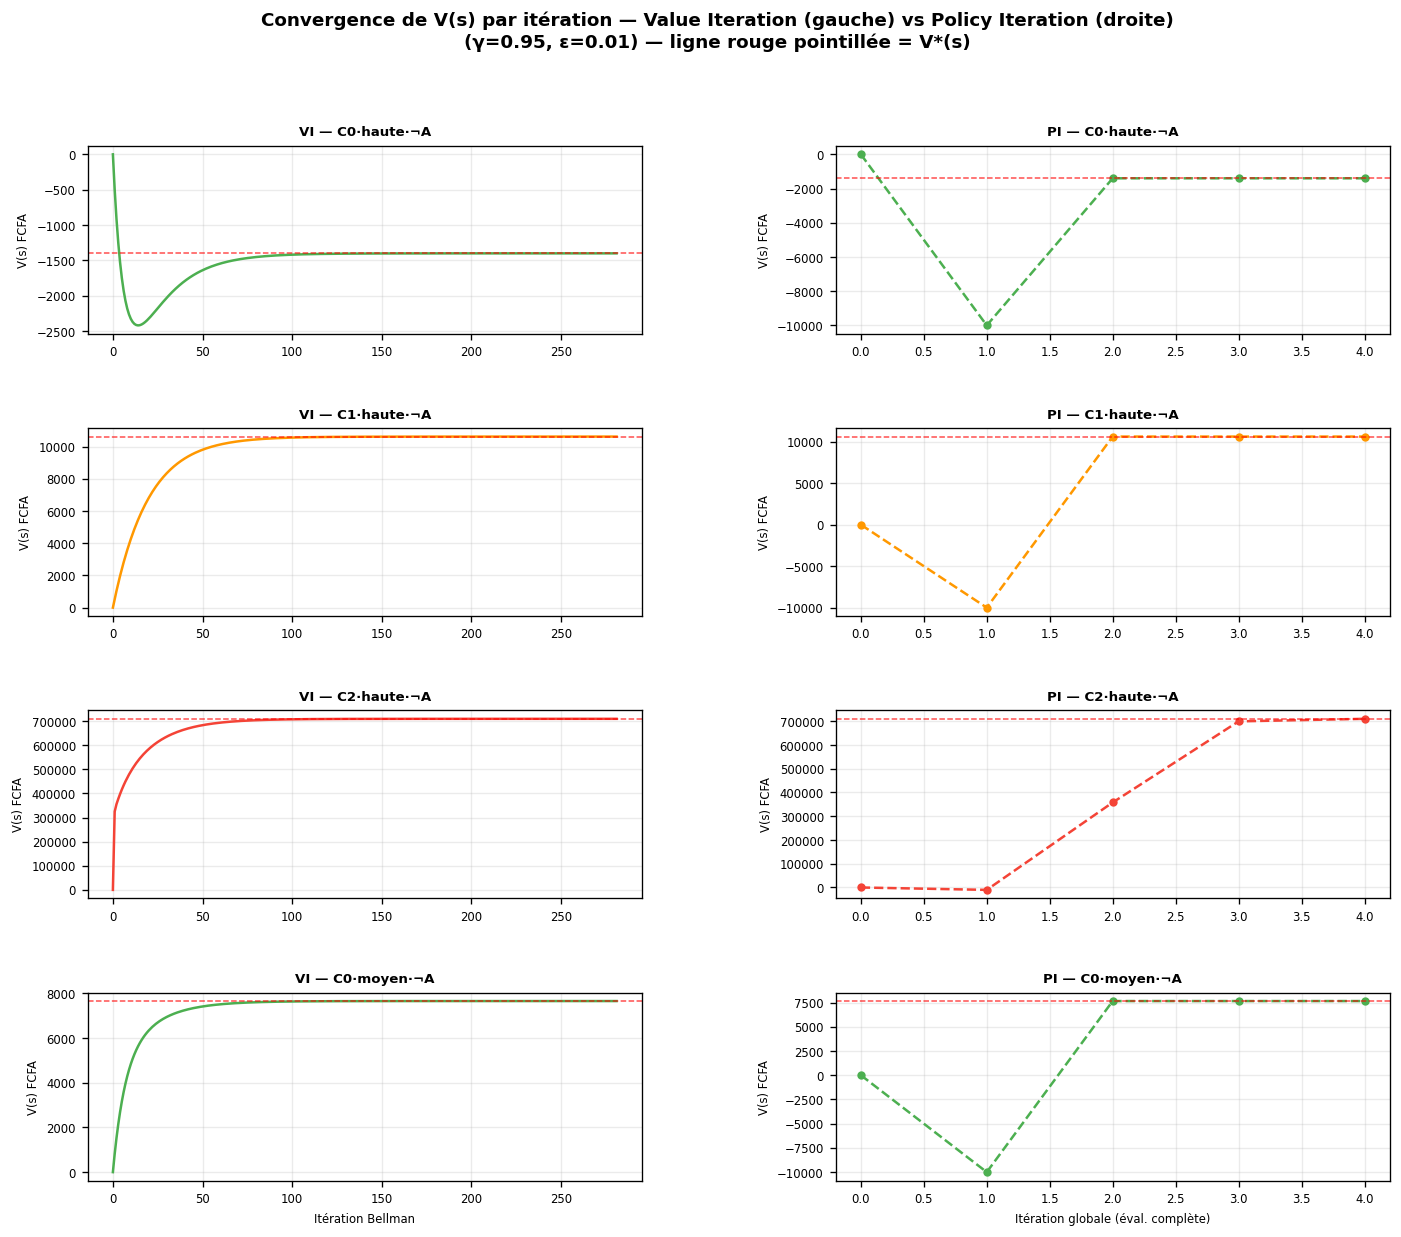
\includegraphics[width=\textwidth]{figures/vi_pi_convergence_states.png}
}{[Figure vi\_pi\_convergence\_states.png absente --- ex\'{e}cuter compare\_vi\_pi.py]}
\caption{Convergence de $V(s)$ par it\'{e}ration --- VI (gauche) vs PI (droite)}
\label{fig:c:vi_pi_states}
\end{figure}

\begin{figure}[H]
\centering
\IfFileExists{figures/vi_pi_comparison_summary.png}{
  
\includegraphics[width=\textwidth]{figures/vi_pi_comparison_summary.png}
}{[Figure vi\_pi\_comparison\_summary.png absente --- ex\'{e}cuter compare\_vi\_pi.py]}
\caption{Comparaison VI vs PI --- vitesse, temps de calcul et accord politique par $\gamma$}
\label{fig:c:vi_pi_summary}
\end{figure}